% Search for XXXX for places which you need to add your contributions. 

\documentclass{article}
\usepackage{graphicx}

\title{COMP20010 Lab Six: Algorithm Analysis}
\author{James Peach}

\begin{document}
\maketitle

% LAB 6 PART 1
\section{Part~1 Algorithm}
\label{sec:algorithm1}

\subsection{Asymptotic run-time analysis}

My algorithm runs in asymptotic time $O(n * log(n)$. The argument for this follows:

My algorithm has three parts:
\begin{enumerate}
	\item load data into array
	\item sort array
	\item find 90\'th percentile value
\end{enumerate}

The loading of the data from file $O(n)$.

Sorting the array with stdlib quicksort $O(n*log(n))$.

Finding the 90\'th percentile value $O(1)$.

this suggests that the dominating factor is the quicksort.

\subsection{Experiments}
\label{sec:experiments1}
The description of the experiments goes here: 

I tested the algorithm with increasing number of n from $1$ to $10,000,000$ 
in powers of $10$.

% If you put your results in a graph, uncomment the following. 

 \begin{figure}
   \centering
 \resizebox{0.9\textwidth}{!}{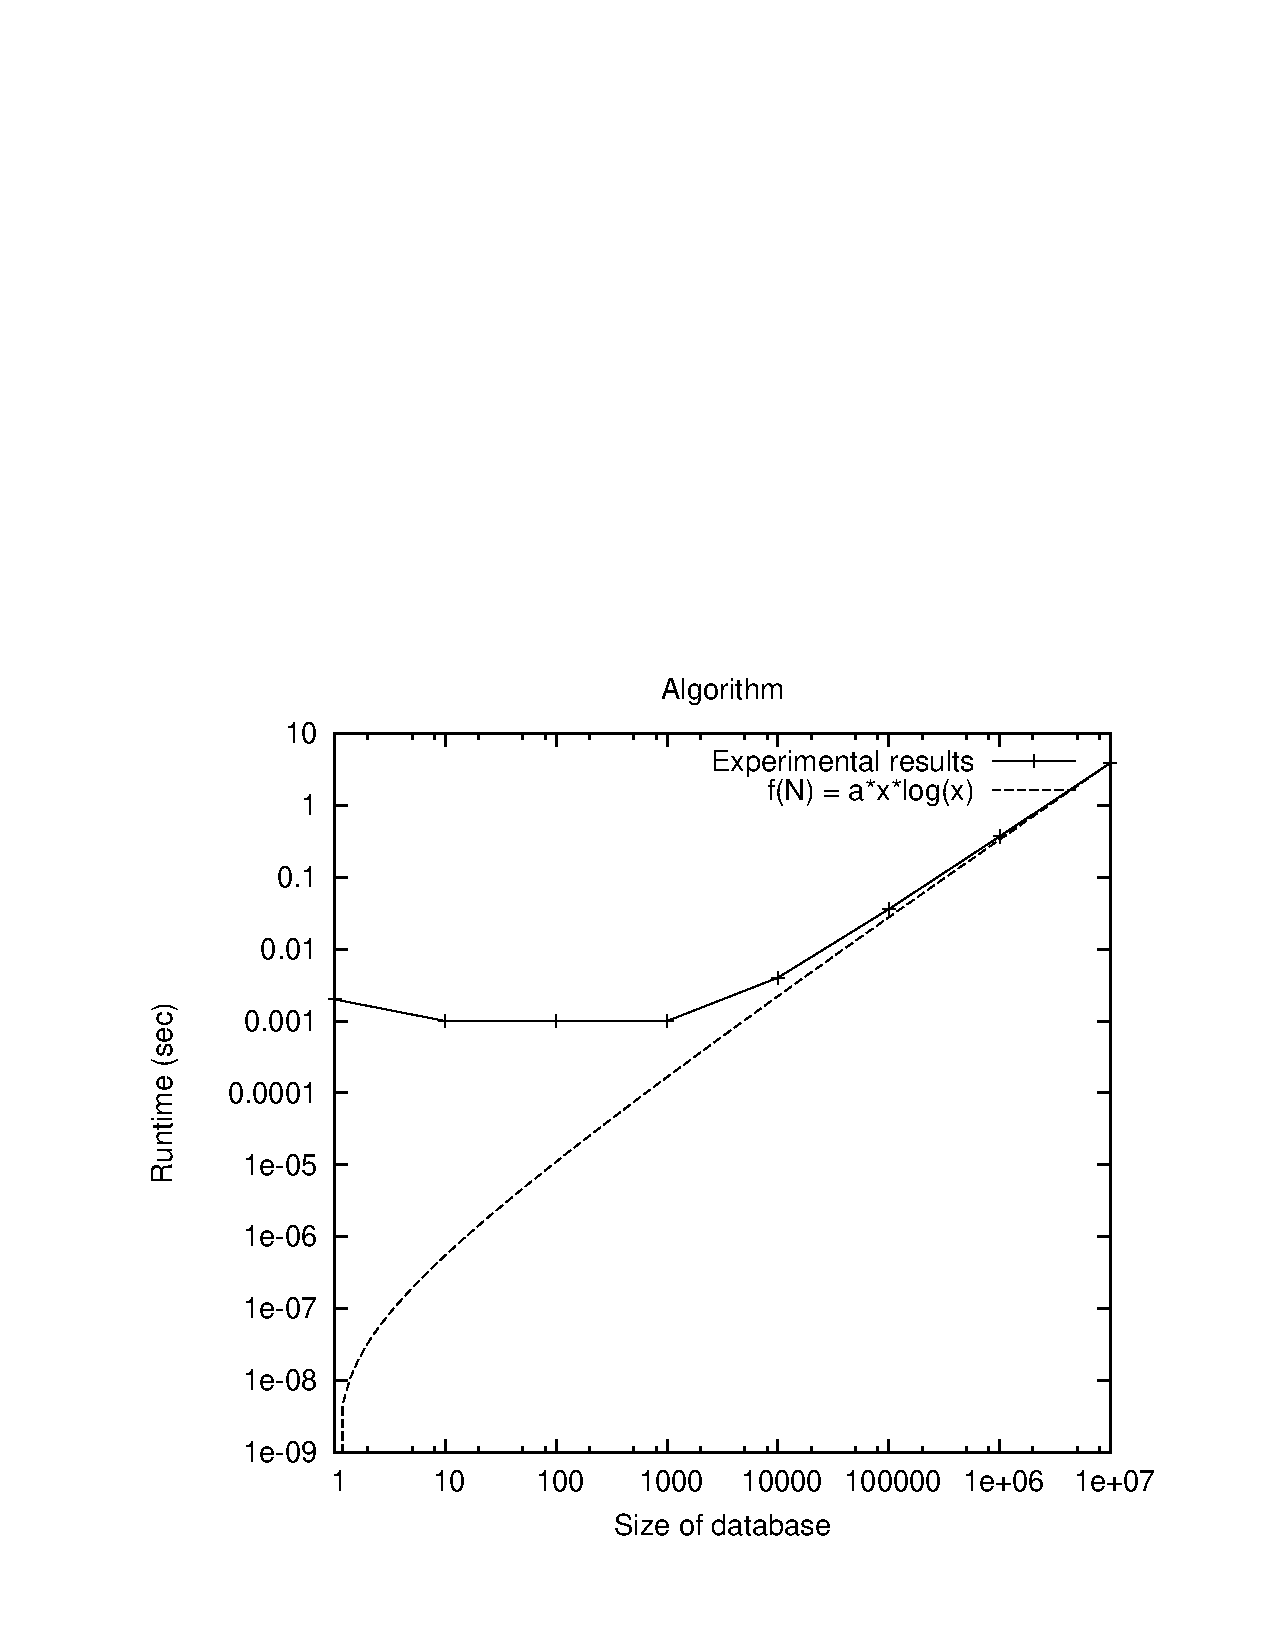
\includegraphics[trim=0cm 0cm 0cm 5cm]{graph-datapoints.pdf}}  
  
   \caption{Real time vs count of numbers}
   \label{fig:experiment1}
 \end{figure}

\subsection{Prediction}
\label{sec:prediction1}

My estimate of the equation for the run-time of the algorithm is:
\begin{equation}
  \label{eq:estimated_runtime1}
  t(N) = 2.4 \times 10^{-8}*log(n)
\end{equation}
Using this, the estimated time to find the ninetieth percentile of a
file containing 60 million numbers is $25.79$ seconds.

%LAB 6 PART 2
\section{Part~2 Algorithm}
\label{sec:algorithm2}

\subsection{Asymptotic run-time analysis}

My algorithm runs in asymptotic time $O(n)$. 

The argument for this follows:

My algorithm has three parts:
\begin{enumerate}
	\item load data into array
	\item sort array
	\item find 90\'th percentile value
\end{enumerate}

The loading of the data from file $O(n)$.

Sorting the array with bucket sort $O(k + k)$.

Finding the 90\'th percentile value $O(1)$.

This suggests that the dominating factor is the sort.


\subsection{Experiments}
\label{sec:experiments2}
The description of the experiments goes here: same as above:

I tested the algorithm with increasing number of n from $1$ to $10,000,000$ 
in powers of $10$.

% If you put your results in a graph, uncomment the following. 


 \begin{figure}
   \centering
 \resizebox{0.9\textwidth}{!}{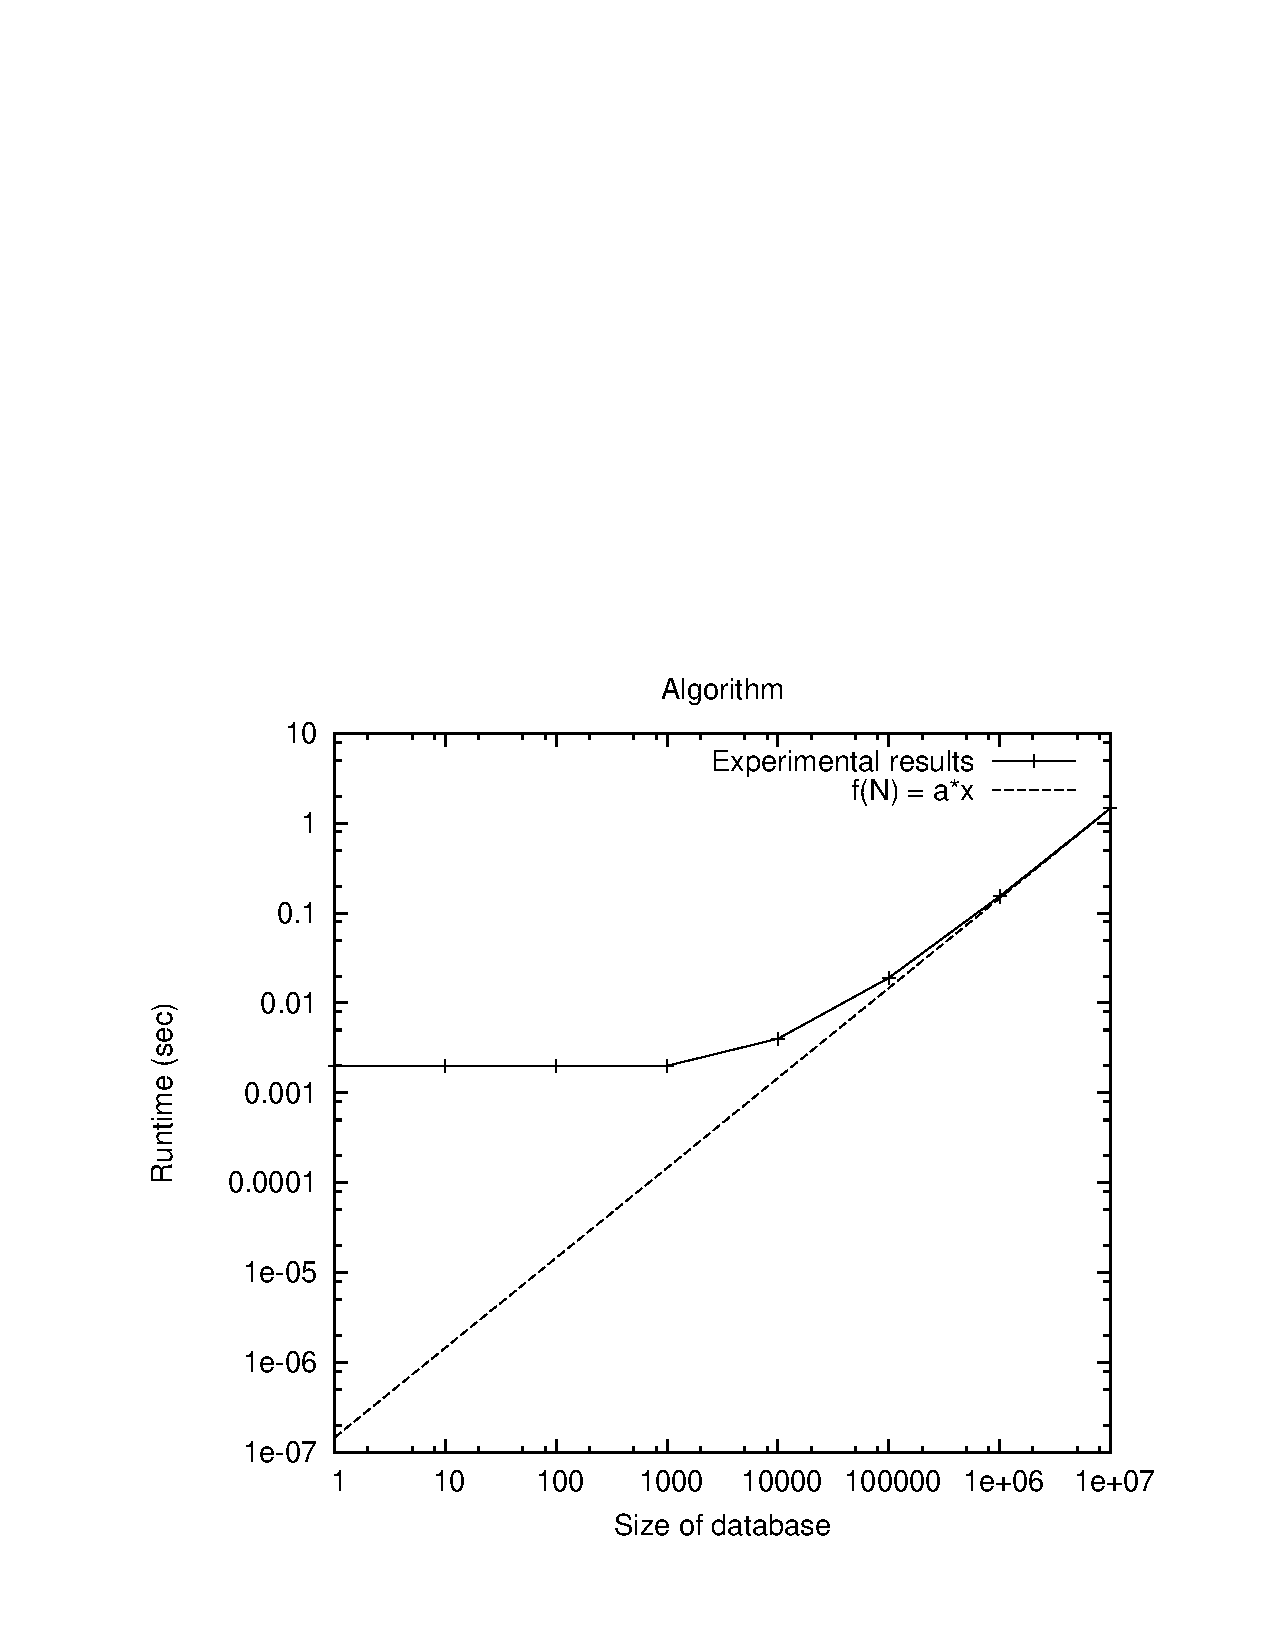
\includegraphics[trim=0cm 0cm 0cm 5cm]{graph-improved.pdf}}  
  
   \caption{Real time vs count of numbers}
   \label{fig:experiment1}
 \end{figure}

% If you put your results in a table, the followin might be helpful. 
% Replace the formula in the third column with the formula you are testing. 

\subsection{Prediction}
\label{sec:prediction2}

My estimate of the equation for the run-time of the algorithm is:
\begin{equation}
  \label{eq:estimated_runtime2}
  t(N) = 1.46*10^{-7} * n
\end{equation}
Using this, the estimated time to find the ninetieth percentile of a
file containing 60 million numbers is $12.8$ seconds.



\end{document}
